\section{The Dwelling Prepared at Sinai}
\label{sec:dwelling-prepared}

At Mount Sinai, immediately after forbidding Israel to carve any graven likeness of the unseen God, the Lord commands Moses to build Him a dwelling. The order of the command is astonishing. God does not begin with the outer hangings of the courtyard, nor with the brazen altar where victims will burn, nor even with the acacia boards of the Tent of Meeting. He begins at the innermost heart of the sanctuary and builds outward from a single chest: ``Frame an ark of setim wood, the length whereof shall be of two cubits and a half; the breadth, a cubit and a half; the height, likewise, a cubit and a half'' (Exod 25:10). Every veil, lamp, silver socket, and priestly vestment in the chapters that follow exists to shelter this chest and to govern how sinful men draw near to the Holy One who speaks above it.

Israel's sanctuary therefore stands apart from every temple of Egypt, Canaan, and Mesopotamia. Those nations raised stone houses to shelter an idol of stone, wood, or gold. The Lord who spoke to Israel from the midst of fire (Deut 10:4) permits no image of Himself, yet wills to dwell genuinely in the midst of His people. At the center of His house He places an empty throne of pure gold, resting over a wooden chest holding the tablets of His covenant and shaded by the wings of hammered cherubim.

The Church confesses that this economy of Sinai reaches its fulfillment in the Incarnation of the eternal Son. Jesus Christ is the eternal Word made flesh, the New Covenant in His blood, and the Presence of the living God in person. Because the Son of God truly took human flesh in the womb of the Blessed Virgin Mary and was borne by her, the Church honors Mary as the living Ark of the New Covenant (\textit{Foederis arca}). Her dignity is wholly created, wholly graced, and ordered without remainder to the Lord who dwelt within her. As St.\ Ambrose states in \textit{On the Holy Spirit} (III.11.80), Mary was the temple of God, not the God of the temple; adoration belongs to Him alone who worked within her.

\subsection{Acacia, Pure Gold, and the Unremoved Poles}
\label{subsec:acacia-gold-poles}

During his forty days and forty nights upon Mount Sinai (Exod 24:18), Moses receives the exact pattern of the Ark before any other vessel of worship is named:

\begin{scriptureblock}
Frame an ark of setim wood, the length whereof shall be of two cubits and a half; the breadth, a cubit and a half; the height, likewise, a cubit and a half. And thou shalt overlay it with the purest gold, within and without; and over it thou shalt make a golden crown round about: And four golden rings, which thou shalt put at the four corners of the ark: let two rings be on the one side, and two on the other. Thou shalt make bars also of setim wood, and shalt overlay them with gold. And thou shalt put them in through the rings that are in the sides of the ark, that it may be carried on them: And they shall be always in the rings, neither shall they at any time be drawn out of them. And thou shalt put in the ark the testimony which I will give thee. \textnormal{(Exod 25:10--16)}
\end{scriptureblock}

After the sin of the golden calf and the renewal of the covenant, the craftsman Bezalel (\textit{Beseleel}), filled with the Spirit of God in wisdom and understanding (Exod 31:2--5), carries out every specification to the letter (Exod 37:1--5; placed in the Septuagint's reordered tabernacle construction narrative at Exod 38:1--4): ``And Beseleel made also, the ark of setim wood: it was two cubits and a half in length, and a cubit and a half in breadth, and the height was of one cubit and a half: and he overlaid it with the purest gold within and without'' (Exod 37:1).

Every proportion and material carries deliberate meaning. Two and a half cubits long, a cubit and a half broad, and a cubit and a half high yield a vessel of human scale---compact enough to ride upon the shoulders of four Levites through mountain passes, yet large enough to hold the two stone tablets of Sinai and to bear a solid golden throne-cover above it. Ancient Near Eastern cubit standards varied slightly, so Exodus fixes exact internal ratios rather than a modern linear measure.

The chest itself joins two distinct substances: \textit{setim} wood (the dense, thorny desert acacia native to Sinai) and ``the purest gold'' (\textit{auro mundissimo}). Acacia wood resists insects and rot in arid country, which led the Greek translators of the Septuagint to render it by an adjective denoting incorruptible timber. Yet Bezalel does not leave even this durable wood exposed. He clads it ``within and without'' (\textit{intus et foris}, Exod 25:11; \textit{intus ac foris}, Exod 37:1) with purest gold, so that the hidden interior holding the tablets matches the exterior facing the cherubim. Holiness in Israel's sanctuary admits no gilded facade; the unseen inside must be as spotless as the face turned outward.

In this union of incorruptible wood and spotless gold, the Fathers contemplated first the Incarnation---sinless human flesh united without confusion to uncreated Divinity---and, in ordered subordination, the unstained humanity of the Virgin in whom the Holy Spirit formed the Lord's dwelling. Commenting on the heavenly Ark of Revelation 11:19, Venerable Bede likens the Divinity dwelling in Christ's holy body to the heavenly manna kept in clean gold. In the Apostolic Constitution \textit{Ineffabilis Deus} (8 December 1854), Pope Pius IX likewise gathers the patristic testimony that the Holy Spirit---the new Bezalel---formed Mary's unstained flesh as a living tabernacle adorned and woven with gold.

Around the upper rim of the chest Bezalel sets a molded golden crown (\textit{coronam auream per circuitum}, Exod 25:11; \textit{per gyrum}, Exod 37:2), both dignifying the chest as a royal footstool and forming a secure ledge for the heavy golden lid during desert marches. Four cast golden rings are affixed at the four corners, two on each side, receiving two gold-clad acacia poles (\textit{vectes}). Over those poles the Lord lays a perpetual ordinance: ``And they shall be always in the rings, neither shall they at any time be drawn out of them'' (Exod 25:15). Two truths meet in that prohibition. First, human hands must never grasp the chest itself; even its appointed bearers carry it solely by the poles on their shoulders. Second, Israel's sanctuary is intrinsically pilgrim and mobile. Unlike territorial idols bolted inside brick shrines, the Lord journeys before His redeemed people across wilderness and river. Even four centuries later, when Solomon installs the Ark inside the cedar-lined inner room of the Jerusalem Temple, the poles remain in the rings, their ends pressing visibly forward before the oracle (1 Kgs 8:8 [Douay-Rheims 3 Kgs 8:8]; 2 Chr 5:9 [2 Par 5:9]).

\subsection{The Propitiatory, the Cherubim, and the Empty Throne}
\label{subsec:propitiatory-cherubim}

Above the acacia chest sits a separate plate of solid gold, matching the length and breadth of the box beneath it:

\begin{scriptureblock}
Thou shalt make also a propitiatory of the purest gold: the length thereof shall be two cubits and a half, and the breadth a cubit and a half. Thou shalt make also two cherubims of beaten gold, on the two sides of the oracle. Let one cherub be on the one side, and the other on the other. Let them cover both sides of the propitiatory, spreading their wings, and covering the oracle, and let them look one towards the other, their faces being turned towards the propitiatory wherewith the ark is to be covered. In which thou shalt put the testimony that I will give thee. Thence will I give orders, and will speak to thee over the propitiatory, and from the midst of the two cherubims, which shall be upon the ark of the testimony, all things which I will command the children of Israel by thee. \textnormal{(Exod 25:17--22)}
\end{scriptureblock}

In Hebrew this solid gold cover is the \textit{kapporet}, a term rooted in covering and atoning for sin; the Septuagint translates it as \textit{hilasterion} (``place of propitiation''), and the Vulgate renders it \textit{propitiatorium} (``propitiatory,'' traditionally also called the mercy seat) while naming it \textit{oraculum} (``the oracle,'' Exod 25:18, 20; 37:6).

It is, first, the meeting place of divine justice and mercy. Inside the chest lie the stone tablets of the Law that expose human transgression; on the Day of Atonement, the high priest enters behind the inner veil and sprinkles sacrificial blood upon and before the golden propitiatory (Lev 16:14--15), interposing blood between the accusing Law below and the glory of God above. St.\ Paul applies the exact Greek noun \textit{hilasterion} to Christ Himself, ``[w]hom God hath proposed to be a propitiation, through faith in his blood'' (Rom 3:25).

It is, second, the speaking-place of God. Exodus 37:6 states the equivalence explicitly: ``He made also the propitiatory, that is, the oracle, of the purest gold.'' Once the Tabernacle stands consecrated, Numbers confirms the promise fulfilled:

\begin{scriptureblock}
And when Moses entered into the tabernacle of the covenant, to consult the oracle, he heard the voice of one speaking to him from the propitiatory, that is over the ark between the two cherubims, and from this place he spoke to him. \textnormal{(Num 7:89)}
\end{scriptureblock}

Hammered from gold (\textit{ex auro ductili}, Exod 37:7) at either end of the propitiatory, the two cherubim face one another across the golden plate with their faces turned downward toward the mercy seat and their wings arched high above it. In Brenton's translation of the Septuagint, Exodus 25:20 and 38:8 (= Vulgate 37:9) describe them as ``overshadowing the propitiatory with their wings.'' The Epistle to the Hebrews preserves that exact gesture in Greek: ``And over it were the cherubims of glory overshadowing the propitiatory'' (Heb 9:5; Vulgate \textit{cherubim gloriae obumbrantia propitiatorium}). The Greek verb of Hebrews 9:5, \textit{kataskiazo} (``to cast a shadow over,'' ``to overshadow''), occurs nowhere else in the entire New Testament and shares its root with \textit{episkiazo}, the verb Gabriel speaks to Mary at Nazareth (Luke 1:35).

Above those wings rests no carved figure. Israel's inner sanctuary holds an empty throne because the Lord who sits ``upon the cherubims'' (1 Sam 4:4 [Douay-Rheims 1 Kgs 4:4]; 2 Sam 6:2 [2 Kgs 6:2]) is uncontained by heaven and earth. Commenting on Psalm 131(132):7--8, St.\ Robert Bellarmine explains that within the sanctuary the Ark formed the Lord's footstool and the propitiatory His seat supported by the two cherubim; Israel addressed God not as confined in His essence---whom the heaven of heavens cannot contain---but as peculiarly present to give His answers from the Ark.

\ifdefined\TriptychPrintEdition
\Needspace{34\baselineskip}
\begin{center}
\begin{tikzpicture}
  \node[anchor=south west, inner sep=0] (img) at (0,0) {%
    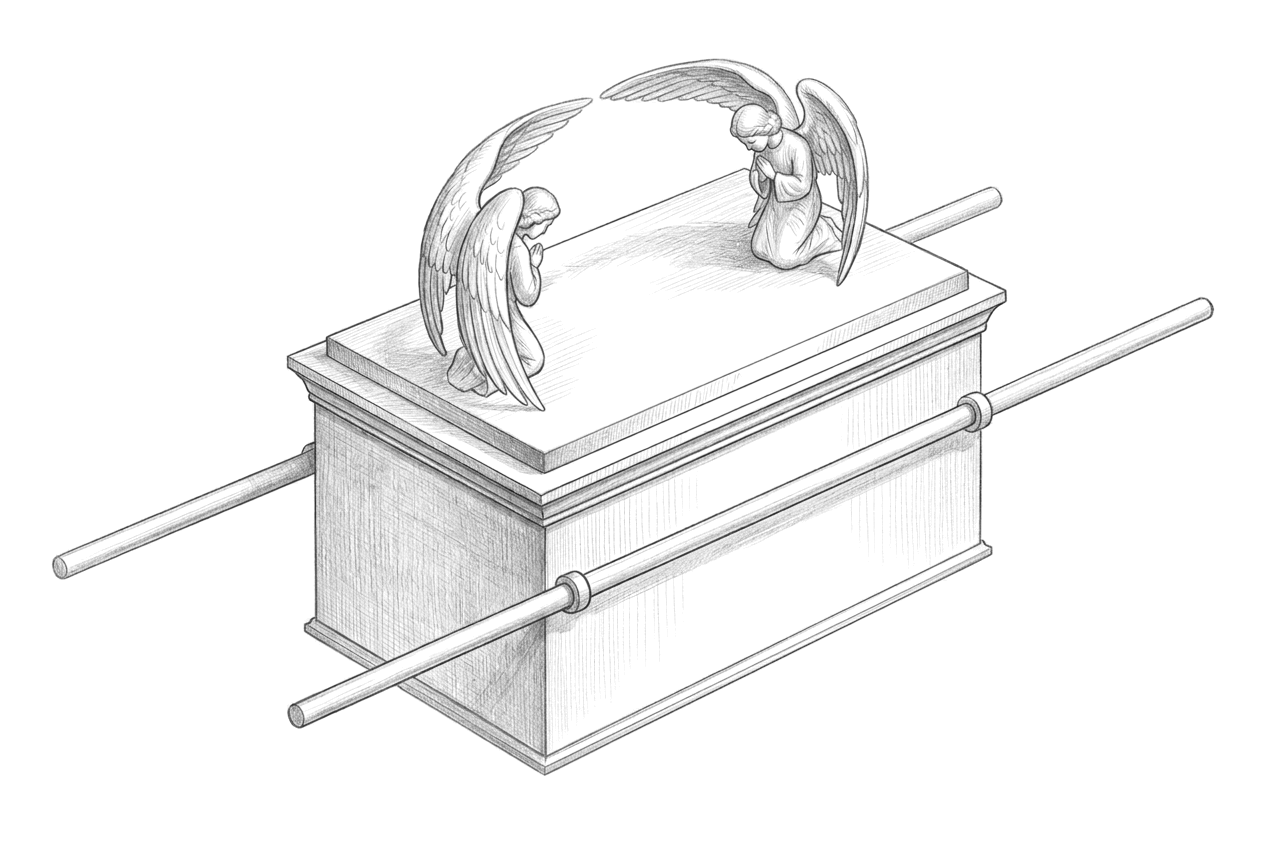
\includegraphics[width=0.90\linewidth]{theology/mariology/ark-of-the-covenant/artwork/ark-anatomy-graphite.png}%
  };
  \begin{scope}[x={(img.south east)}, y={(img.north west)}]
    \node[font=\scriptsize, fill=white, inner sep=1.5pt] (c1) at (0.24, 0.90) {Two hammered cherubim};
    \draw[draw=black!65, line width=0.4pt] (c1) -- (0.38, 0.84);
    \fill[black!75] (0.38, 0.84) circle (1.1pt);

    \node[font=\scriptsize, fill=white, inner sep=1.5pt] (c2) at (0.76, 0.91) {Overshadowing wings};
    \draw[draw=black!65, line width=0.4pt] (c2) -- (0.58, 0.90);
    \fill[black!75] (0.58, 0.90) circle (1.1pt);

    \node[font=\scriptsize, fill=white, inner sep=1.5pt] (c3) at (0.84, 0.77) {Propitiatory (mercy seat)};
    \draw[draw=black!65, line width=0.4pt] (c3) -- (0.55, 0.65);
    \fill[black!75] (0.55, 0.65) circle (1.1pt);

    \node[font=\scriptsize, fill=white, inner sep=1.5pt] (c4) at (0.15, 0.69) {Molded crown of gold};
    \draw[draw=black!65, line width=0.4pt] (c4) -- (0.27, 0.59);
    \fill[black!75] (0.27, 0.59) circle (1.1pt);

    \node[font=\scriptsize, fill=white, inner sep=1.5pt] (c5) at (0.80, 0.23) {Acacia chest overlaid with gold};
    \draw[draw=black!65, line width=0.4pt] (c5) -- (0.65, 0.34);
    \fill[black!75] (0.65, 0.34) circle (1.1pt);

    \node[font=\scriptsize, fill=white, inner sep=1.5pt] (c6) at (0.17, 0.13) {Four rings and unremoved poles};
    \draw[draw=black!65, line width=0.4pt] (c6) -- (0.45, 0.30);
    \fill[black!75] (0.45, 0.30) circle (1.1pt);
  \end{scope}
\end{tikzpicture}
\end{center}\nopagebreak[4]
\else
\begin{studybox}{Plate I: Architectural Anatomy of the Ark of the Covenant}
Viewed in three-quarter isometric elevation, the Ark unites six coordinated parts commanded in Exodus 25:10--22 and crafted by Bezalel in Exodus 37:1--9:
\begin{itemize}
  \item \textbf{Acacia chest overlaid with gold:} A rectangular chest proportioned at 2.5 cubits long, 1.5 cubits broad, and 1.5 cubits high, framed of \textit{setim} (acacia) wood and overlaid within and without with pure gold.
  \item \textbf{Molded crown of gold:} A raised golden rim running around the upper perimeter of the chest, dignifying the vessel and seating its cover securely.
  \item \textbf{Four rings and unremoved poles:} Four cast golden rings affixed at the four corners (two on each long side), holding two continuous gold-clad acacia bars that remain permanently inserted so the Ark may be borne on Levitical shoulders without direct touch.
  \item \textbf{Propitiatory (mercy seat):} A solid slab of purest gold (2.5 by 1.5 cubits) closing the top of the chest as the place of atonement and divine oracle.
  \item \textbf{Two hammered cherubim:} Two golden angelic figures rising from the opposite ends of the propitiatory, facing one another with bowed heads and eyes directed downward toward the mercy seat.
  \item \textbf{Overshadowing wings:} High arched wings stretched forward from both cherubim to canopy the unoccupied throne-space above the propitiatory where the Lord speaks to Moses.
\end{itemize}
\end{studybox}
\fi
\begin{platecaption}
\textbf{Plate I. Architectural anatomy of the Ark of the Covenant (Exod 25:10--22; 37:1--9).} Exodus prescribes the proportions (2.5 by 1.5 by 1.5 cubits), the pure-gold overlay inside and out, the golden crown molding, the four corner rings with permanent carrying poles, the solid gold propitiatory, and the two hammered cherubim facing one another with bowed gaze and overshadowing wings. Because ancient cubit standards varied and Scripture does not describe the precise anatomy or posture of the cherubim, the sculpted figures represent an illustrative architectural rendering rather than an archaeological reconstruction.
\end{platecaption}

\subsection{What Rested Within, Before, and Beside the Ark}
\label{subsec:contents-of-ark}

Across the Old and New Testaments, four sacred memorials belong to the Ark's immediate compass: the stone tablets of the Decalogue, the vessel of manna, Aaron's blossomed rod, and the scroll of the Law. Scripture distinguishes with care what rested inside the chest from what was laid before or beside it.

\subsubsection{Within the Ark: The Tablets of the Testimony}

In the Mosaic legislation, only one deposit is explicitly commanded to be placed inside the acacia chest: the two stone tablets of the Ten Commandments, called ``the testimony'' (\textit{testificationem}, Exod 25:16; \textit{testimonium}, Exod 25:21). In Deuteronomy 10:1--5, Moses recalls hewing two new stone tablets after breaking the first pair at the foot of Sinai, ascending the mount again, receiving ``the ten words, which the Lord spoke to you in the mount from the midst of the fire'' (Deut 10:4), and setting them directly inside the chest: ``And returning from the mount, I came down, and put the tables into the ark, that I had made, and they are there till this present, as the Lord commanded me'' (Deut 10:5).

Four centuries later, when King Solomon transfers the Ark from David's tent on Zion into the inner oracle of the Jerusalem Temple, both 1 Kings 8:9 and 2 Chronicles 5:10 confirm the sole contents inside the chest:

\begin{scriptureblock}
Now in the ark there was nothing else but the two tables of stone, which Moses put there at Horeb, when the Lord made a covenant with the children of Israel, when they came out of the land of Egypt. \textnormal{(1 Kgs 8:9)}
\end{scriptureblock}

Because those second stone tablets restored what Israel's sin had shattered, the Fathers saw in them a figure of human nature broken by Adam's fall and formed anew by the Holy Spirit in Mary's womb. Commenting on Luke 1:35, St.\ Gregory of Nyssa (in his \textit{Life of Moses}, preserved in St.\ Thomas Aquinas's \textit{Catena Aurea in Lucam}) writes:

\begin{quote}\small
For the tables of our nature which guilt had broken, the true Lawgiver has formed anew Himself from our dust without cohabitation, creating a body capable of taking His divinity, which the finger of God hath carved, that is to say, the Spirit coming upon the Virgin.
\end{quote}

\subsubsection{Before and Beside the Ark in the Pentateuch}

Beside the tablets within the chest, the Pentateuch appoints three further memorials to be kept immediately before or alongside the Ark:

\begin{itemize}
  \item \textbf{The vessel of manna (Exod 16:33--34):} When heavenly bread first falls in the wilderness, Moses instructs Aaron: ``Take a vessel, and put manna into it, as much as a gomor can hold; and lay it up before the Lord, to keep unto your generations, As the Lord commanded Moses. And Aaron put it in the tabernacle to be kept.'' Where the Vulgate reads \textit{vas unum} (``a vessel'') placed \textit{in tabernaculo} (``in the tabernacle''), Brenton's Septuagint specifies ``a golden pot'' laid up ``before the testimony''---preserving the exact detail of a golden vessel that reappears in the Epistle to the Hebrews.
  \item \textbf{Aaron's blossomed rod (Num 17:10; LXX 17:25):} After Korah's rebellion challenges the priesthood, Aaron's dry almond staff sprouts buds, flowers, and ripe almonds overnight before the testimony. The Lord commands Moses: ``Carry back the rod of Aaron into the tabernacle of the testimony, that it may be kept there for a token of the rebellious children of Israel, and that their complaints may cease from me lest they die'' (Num 17:10; Brenton's Septuagint, numbered 17:25, reads ``before the testimonies'').
  \item \textbf{The book of the law (Deut 31:24--26):} Completing his final scroll of the Law, Moses delivers it to the Levites who carry the Ark: ``Take this book, and put it in the side of the ark of the covenant of the Lord your God: that it may be there for a testimony against thee'' (Deut 31:26; Vulgate \textit{in latere arcae}).
\end{itemize}

\subsubsection{Hebrews 9:4 and the Threefold Fulfillment in Christ}

Looking back upon the ordering of the first sanctuary, the Epistle to the Hebrews gathers the golden pot of manna, Aaron's blossomed rod, and the stone tablets into one solemn inventory:

\begin{scriptureblock}
And after the second veil, the tabernacle which is called the Holy of Holies: Having a golden censer and the ark of the testament covered about on every part with gold, in which was a golden pot that had manna and the rod of Aaron that had blossomed and the tables of the testament. And over it were the cherubims of glory overshadowing the propitiatory: of which it is not needful to speak now particularly. \textnormal{(Heb 9:3--5)}
\end{scriptureblock}

Catholic exegesis harmonizes Hebrews 9:4 (``in which,'' \textit{in qua}) with 1 Kings 8:9 along two complementary lines. First, Hebrews 9 expressly describes ``the first'' or wilderness tabernacle (Heb 9:2, 8), not Solomon's Temple four hundred years later, after the Ark had endured capture in Philistia and decades of displacement outside Shiloh. Second, traditional commentators understand the phrasing of Hebrews to gather the entire sacred ensemble resting within and immediately adjoining the chest inside the Holy of Holies. Bishop Richard Challoner states this classical harmony directly in his footnote on 1 Kings 8:9 (3 Kings in the Douay-Rheims):

\begin{quote}\small
There was nothing else but the tables of the law within the ark: but on the outside of the ark, or near the ark were also the rod of Aaron, and a golden urn with manna, Heb. 9.4.
\end{quote}

\begin{threestable}{Sacred Deposit}{Scriptural Placement}{Fulfillment in Christ}
Two tables of stone & Inside the Ark (Exod 25:16, 21; Deut 10:2, 5); sole interior contents at Solomon's dedication (1 Kgs 8:9; 2 Chr 5:10); named in Heb 9:4. & Christ the eternal Word and living Law of God, formed anew in human flesh by the Holy Spirit in the Virgin (John 1:14; St.\ Gregory of Nyssa). \\
\addlinespace[0.25em]
Golden pot of manna & Laid up before the Lord / in the tabernacle (Exod 16:33--34; ``a golden pot'' laid ``before the testimony'' in LXX); joined to the Ark in Heb 9:4. & Christ the living Bread come down from heaven, giving His flesh for the life of the world (John 6:31--35, 51; Venerable Bede). \\
\addlinespace[0.25em]
Aaron's blossomed rod & Kept in the tabernacle / before the testimony (Num 17:10 [LXX 17:25]); joined to the Ark in Heb 9:4. & Christ the eternal High Priest (Heb 9:11--12), whose dead wood of the Cross blooms with risen life, sprung from the virginal rod of Jesse. \\
\addlinespace[0.25em]
Book of the Law & Placed ``in the side of the ark'' (\textit{in latere arcae}, Deut 31:26) as a covenant testimony. & The written Law and prophets testifying to the incarnate Son who fulfills them (Matt 5:17; Luke 24:44). \\
\end{threestable}

In Hebrews 9:4, the three signs of the wilderness sanctuary converge into one prophetic portrait of the Redeemer. Under the Old Covenant, those three offices remained separate and inanimate: stone bore the written Law, a golden urn preserved desert bread as a memorial, and a once-flowering almond staff verified a mortal priesthood handed from father to son. In the New Covenant, all three converge in one living Person. Jesus Christ is the eternal Word who writes the New Law upon human hearts; He is the living Bread come down from heaven; He is the eternal High Priest who passes ``by a greater and more perfect tabernacle, not made with hand'' (Heb 9:11) to enter once into the heavenly Holies by His own blood. Because Mary conceived and carried within her immaculate womb the Word, the Bread of Life, and the Eternal High Priest in His own sacred flesh, the ancient chest of Sinai points beyond itself to the living Mother of the Lord.
